% !TeX spellcheck = en_GB
% encoding: utf8
% !TEX encoding = utf8
% !TEX program = pdflatex
% !BIB program = biber

\documentclass[11pt,oneside,a4paper]{report}

\usepackage[utf8]{inputenc}
\usepackage[T1]{fontenc}
\usepackage[colorlinks]{hyperref}
\usepackage[left=2.5cm, right=2.5cm, top=2.5cm, bottom=2.5cm]{geometry}
\usepackage{float}
\usepackage{subcaption}
\usepackage{mathtools}
\usepackage{color}
\usepackage{listings}
\usepackage{xcolor}
\usepackage[backend=biber,maxnames=10,style=numeric,sorting=nty,abbreviate=false,giveninits=true,language=english]{biblatex}

\addbibresource{../meros.bib}

%\newcommand{\twc}[1]{\textcolor{red}{\textbf{TW}: #1}}
\newcommand{\Fig}[1]{Fig.~\ref{#1}}

\definecolor{amber}{rgb}{1.0, 0.49, 0.0}
\newcommand{\twci}[1]{
	\textcolor{amber}{TW: #1}}

% encoding: utf8
%
% Stereotypes
%

% Lista powinna być zgodna z profilem w EA

\newcommand{\stActionConn}{<<Action>>}
\newcommand{\stCommChannel}{<<CommChannel>>}
\newcommand{\stComponContain}{<<ComponContain>>}
\newcommand{\stGpPackages}{<<GpPackages>>}
\newcommand{\stHardware}{<<Hardware>>}
\newcommand{\stLaunchFile}{<<LaunchFile>>}
\newcommand{\stMetaPackage}{<<MetaPackage>>}
\newcommand{\stMicroNode}{<<MicroNode>>}
\newcommand{\stNamespace}{<<Namespace>>}
\newcommand{\stNode}{<<Node>>}
\newcommand{\stPackage}{<<Package>>}
\newcommand{\stParameter}{<<Parameter>>}
\newcommand{\stRepository}{<<Repository>>}
\newcommand{\stRosCommCompon}{<<RosCommCompon>>}
\newcommand{\stRosConn}{<<RosConn>>}
\newcommand{\stRQtNode}{<<RQtNode>>}
\newcommand{\stRunSystemCompon}{<<RunSystemCompon>>}
\newcommand{\stServiceConn}{<<Service>>}
\newcommand{\stSourExeContain}{<<SourExeContain>>}
\newcommand{\stSystem}{<<System>>}
\newcommand{\stTerminal}{<<Terminal>>}
\newcommand{\stTopicConn}{<<Topic>>}
\newcommand{\stWorkspace}{<<Workspace>>}

\newcommand{\stblock}{<<block>>}






\lstdefinestyle{terminal}{
	backgroundcolor=\color{darkgray},
	basicstyle=\ttfamily\color{green}\scriptsize,
	frame=single,
	breaklines=true,
	rulecolor=\color{gray},
}


\begin{document}
	
\title{MeROS 4.0.0: basics of metamodel usage with turtlesim}
\author{MeROS developers group - https://github.com/twiniars/MeROS \\ tomasz.winiarski@pw.edu.pl}
\date{\today}
\maketitle

	
	
	\maketitle
	

	
\chapter*{Important citation notice}

\textbf{If you are to use MeROS in your papers, please first cite the IEEE ACCESS  article~\cite{meros-access}, where the initial version of the MeROS is presented. You can also refer to MeROS project page \cite{meros-www} and mention the actual MeROS version you are using.}
	
\chapter{Introduction}
\label{ch:introduction}

	This document is to present basics of MeROS metamodel usage (its application). It bases on popular turtlesim ROS2 tutorial \url{https://docs.ros.org/en/jazzy/Tutorials/Beginner-CLI-Tools.html} and has an introspection, reverse engineering nature. The procedure of the new systems creation with V-model and MerROS is presented in \cite{winiarski2025-v-model}. We advice to read it after this documentation as the article adds a lot of valuable examples of MeROS related diagrams creation. 

\chapter{MeROS application}
\label{ch:application}

The general scenario is presented in Fig.~\ref{fig:general_scenario_sd}. It is convenient to create the dedicated package in Visual Paradigm (VP) and place the diagrams and other elements inside this package.


\begin{figure}[H]
	\centering
	\begin{center}
		{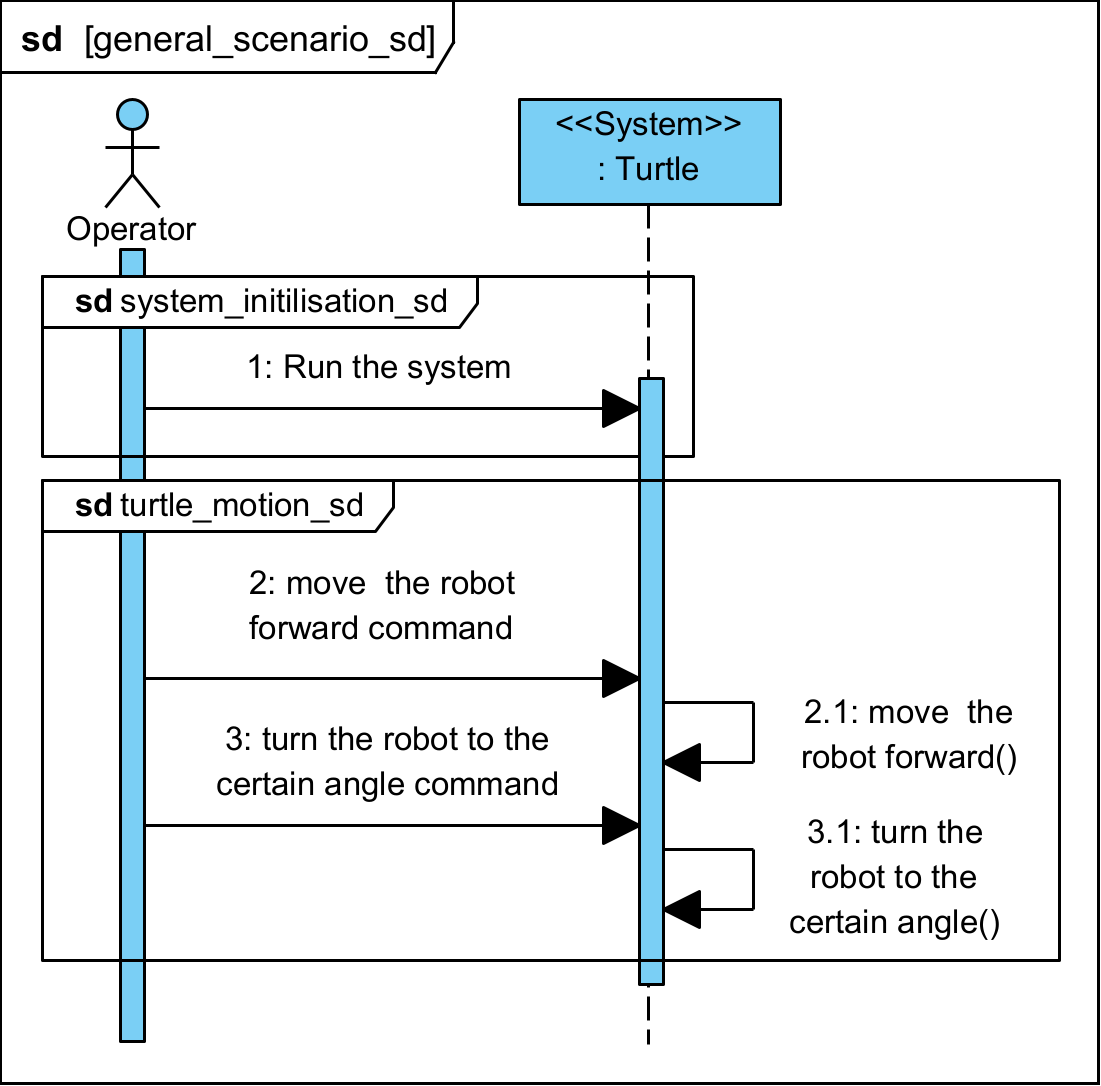
\includegraphics[scale=1.0]{diagrams/general_scenario_sd.png}}
	\end{center}
	\caption{General scenario}
	\label{fig:general_scenario_sd}
\end{figure}


The decision is to build the \stSystem{} comprising two \stNode{}s that are executed. the first is \textsf{turtlesim\_node} \stNode{} from \textsf{turtlesim} \stPackage{}. It should be noted that tourtlesim ROS package should be installed before as well as source command should be executed properly in each system terminal (List.~\ref{lst:ros2_run_turtlesim_turtlesim_node}).

\begin{lstlisting}[style=terminal,label={lst:ros2_run_turtlesim_turtlesim_node},caption={ros2 run turtlesim turtlesim\_node}]
$ ros2 run turtlesim turtlesim_node
[INFO] [1751724881.187110472] [turtlesim]: Starting turtlesim with node name /turtlesim
[INFO] [1751724881.196178869] [turtlesim]: Spawning turtle [turtle1] at x=[5.544445], y=[5.544445], theta=[0.000000]
\end{lstlisting}

The second \stNode{} to be executed, \textsf{turtle\_teleop\_key}, also origins from the \textsf{turtlesim} \stPackage{}. It should be noted that typically new system terminal is needed to execute extra \stNode{} with \textsf{ros2 run} \stCLTool{} (List.~\ref{lst:ros2_run_turtle_teleop_key}).

\begin{lstlisting}[style=terminal,label={lst:ros2_run_turtle_teleop_key},caption={ros2 run turtlesim turtle\_teleop\_key}]
$ ros2 run turtlesim turtle_teleop_key
Reading from keyboard
---------------------------
Use arrow keys to move the turtle.
Use g|b|v|c|d|e|r|t keys to rotate to absolute orientations. 'f' to cancel a rotation.
'q' to quit.
\end{lstlisting}

It is time to draw \stSystem{} structure with \textsf{rqt\_graph} \stCLTool{} (in new system terminal)  (List.~\ref{lst:rqt_graph}). All of the extra elements should be hided, to concentrate on the scenario relevant \stSystem{} components, that are also considered in the following diagrams.

\begin{lstlisting}[style=terminal,label={lst:rqt_graph},caption={rqt\_graph}]
$ rqt_graph
\end{lstlisting}

The resultant rosgraph diagram is presented in Fig.~\ref{fig:rqt_graph}. There are two \stNode{}s visible as well as three \stTopic{}s between them. Two of them belong to an \stAction{}.

\begin{figure}[H]
	\centering
	\begin{center}
		{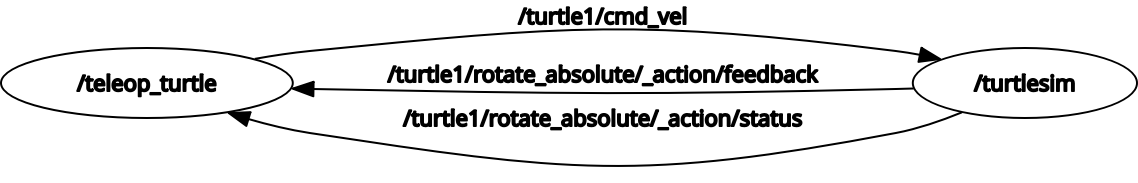
\includegraphics[scale=.5]{diagrams/rosgraph.png}}
	\end{center}
	\caption{System structure by rqt\_graph}
	\label{fig:rqt_graph}
\end{figure}


The MeROS \stSystem{} structure presentation is composed by different views on it. In this example we start with Sources and Executables composition into the \stSystem{}. There are two scenario relevant \stNode{}s to be considered in the in \textsf{Turtle} \stSystem{}. They were run from \textsf{turtlesim} \stPackage{} that can be validated by the \textsf{ros2 pkg} \stCLTool{} (List.~\ref{lst:ros2_pkg_executables_turtlesim}).

\begin{lstlisting}[style=terminal,label={lst:ros2_pkg_executables_turtlesim},caption={ros2 pkg executables turtlesim}]
$ ros2 pkg executables turtlesim
turtlesim draw_square
turtlesim mimic
turtlesim turtle_teleop_key
turtlesim turtlesim_node
\end{lstlisting}

The two extra executables from this \stPackage{} are not considered further on. It is also needed to find the \stPackage{}s containing \stRosConnection{}s used in our example. One of the ways is two find all of the connections for the particular \stNode{} with \textsf{ros2 node} \stCLTool{} (List.~\ref{lst:ros2_node_info_turtlesim}).


\begin{lstlisting}[style=terminal,label={lst:ros2_node_info_turtlesim},caption={ros2 node info /turtlesim}]
$ ros2 node info /turtlesim 
/turtlesim
Subscribers:
/parameter_events: rcl_interfaces/msg/ParameterEvent
/turtle1/cmd_vel: geometry_msgs/msg/Twist
Publishers:
/parameter_events: rcl_interfaces/msg/ParameterEvent
/rosout: rcl_interfaces/msg/Log
/turtle1/color_sensor: turtlesim/msg/Color
/turtle1/pose: turtlesim/msg/Pose
Service Servers:
/clear: std_srvs/srv/Empty
/kill: turtlesim/srv/Kill
/reset: std_srvs/srv/Empty
/spawn: turtlesim/srv/Spawn
/turtle1/set_pen: turtlesim/srv/SetPen
/turtle1/teleport_absolute: turtlesim/srv/TeleportAbsolute
/turtle1/teleport_relative: turtlesim/srv/TeleportRelative
/turtlesim/describe_parameters: rcl_interfaces/srv/DescribeParameters
/turtlesim/get_parameter_types: rcl_interfaces/srv/GetParameterTypes
/turtlesim/get_parameters: rcl_interfaces/srv/GetParameters
/turtlesim/get_type_description: type_description_interfaces/srv/GetTypeDescription
/turtlesim/list_parameters: rcl_interfaces/srv/ListParameters
/turtlesim/set_parameters: rcl_interfaces/srv/SetParameters
/turtlesim/set_parameters_atomically: rcl_interfaces/srv/SetParametersAtomically
Service Clients:

Action Servers:
/turtle1/rotate_absolute: turtlesim/action/RotateAbsolute
Action Clients:
\end{lstlisting}

By taking into account \stRosConnection{}s from Fig.~ \ref{fig:rqt_graph} listed in List.~\ref{lst:ros2_node_info_turtlesim} the \stPackage{}s containing theirs sources can be found as well as 
instances names, used in, e.g. ibd. Finally, taking into account the data presented above, the bdd with \textsf{turtlesim} \stSystem{} sources and containers can be prepared (Fig.~\ref{fig:system_sourexec_composition_bdd}). For that purpose the ROS 2 \stWorkspace{} localisation is needed, but it easy te recognise, especially the initial \textsf{source} command needs it. It is  \textsf{/opt/ros/jazzy} in case of the ROS version used in the time of the creation of this documentation.

\begin{figure}[H]
	\centering
	\begin{center}
		{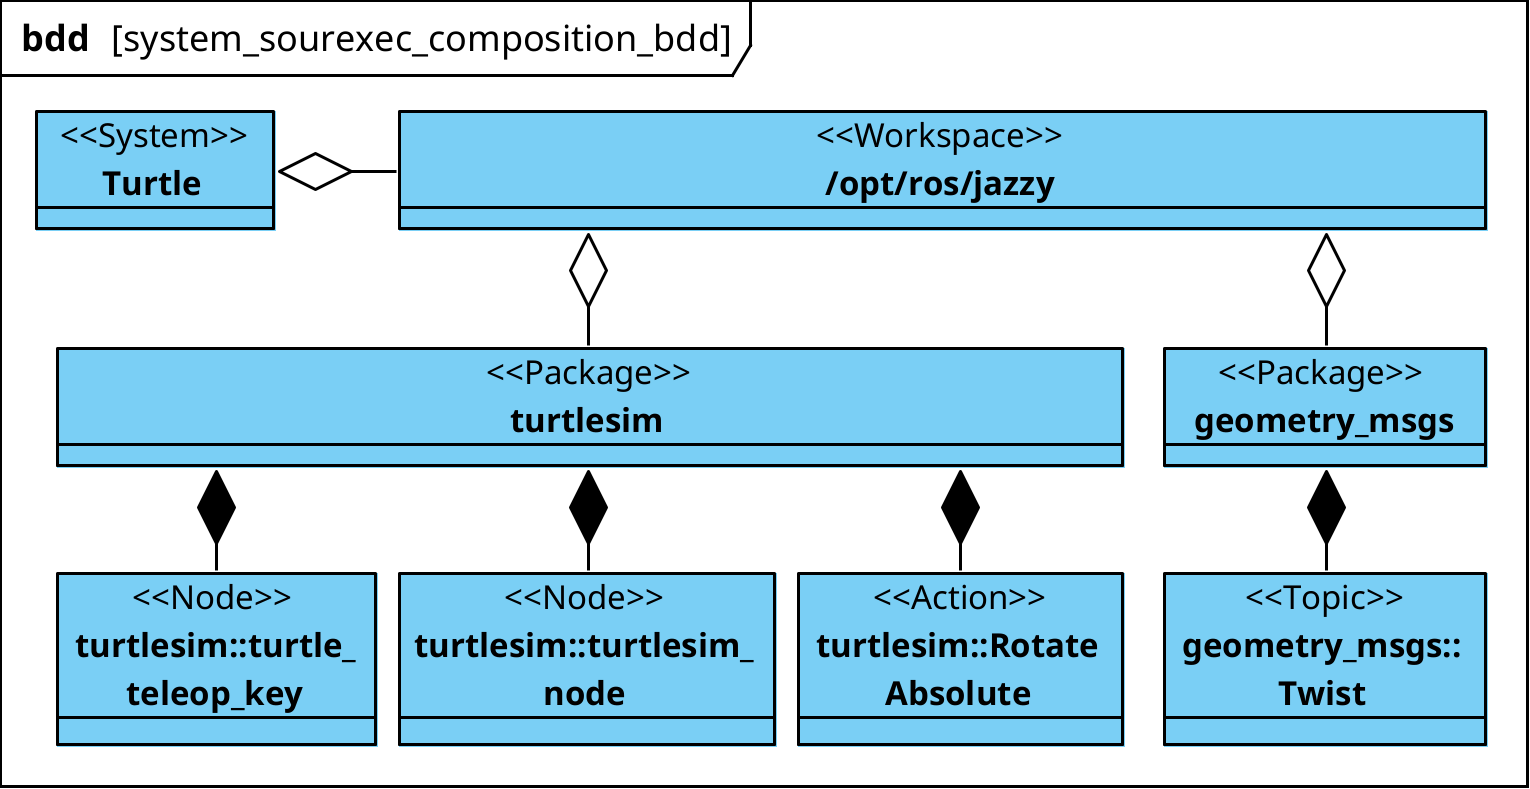
\includegraphics[scale=1.0]{diagrams/system_sourexec_composition_bdd.png}}
	\end{center}
	\caption{System sources and executables composition}
	\label{fig:system_sourexec_composition_bdd}
\end{figure}

As all of the sources and executables are defined for the particular \stPackage{} it is a good practice to take it into account, and define the names of the \stPackage{} parts with the \stPackage{} name at the beginning followed by the double colon. 

Another view on \stSystem{} depicts the running system architecture. It can be depicted in general way. It is needed to first create bdd with all of the elements considered in this view (Fig.~\ref{fig:running_system_general_bdd}).
			
\begin{figure}[H]
	\centering
	\begin{center}
		{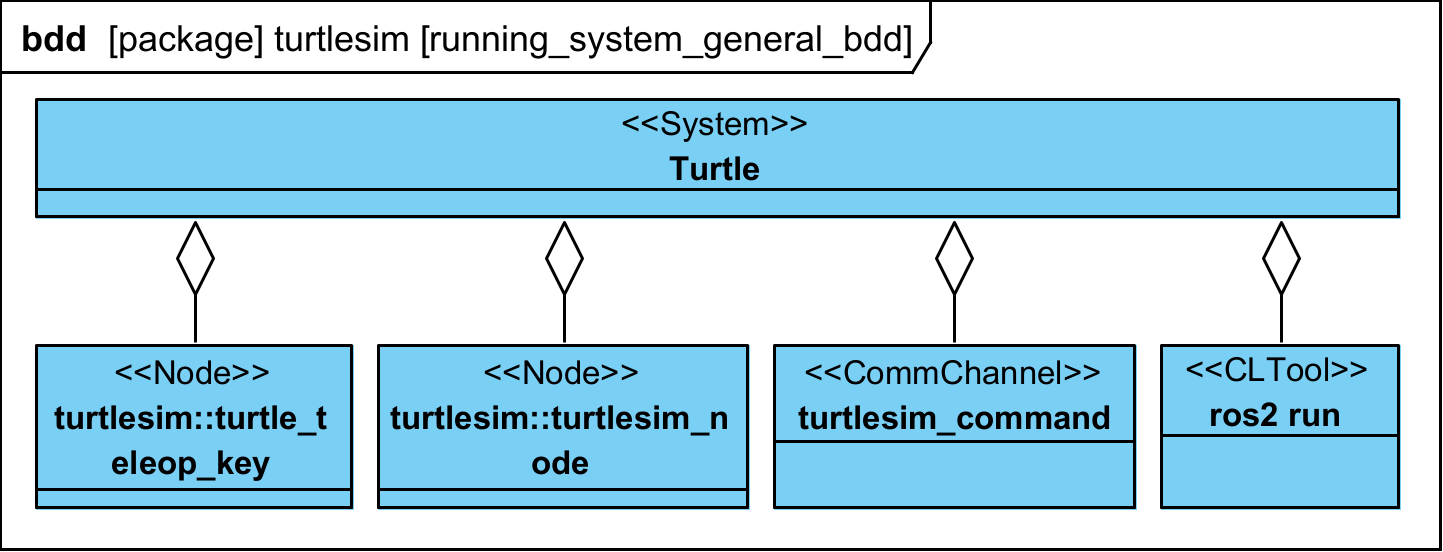
\includegraphics[scale=1.0]{diagrams/running_system_general_bdd.png}}
	\end{center}
	\caption{Running System general view bdd}
	\label{fig:running_system_general_bdd}
\end{figure}

\pagebreak

Then, the ibd can be created (Fig.~\ref{fig:running_system_general_ibd}). 

\begin{figure}[H]
	\centering
	\begin{center}
		{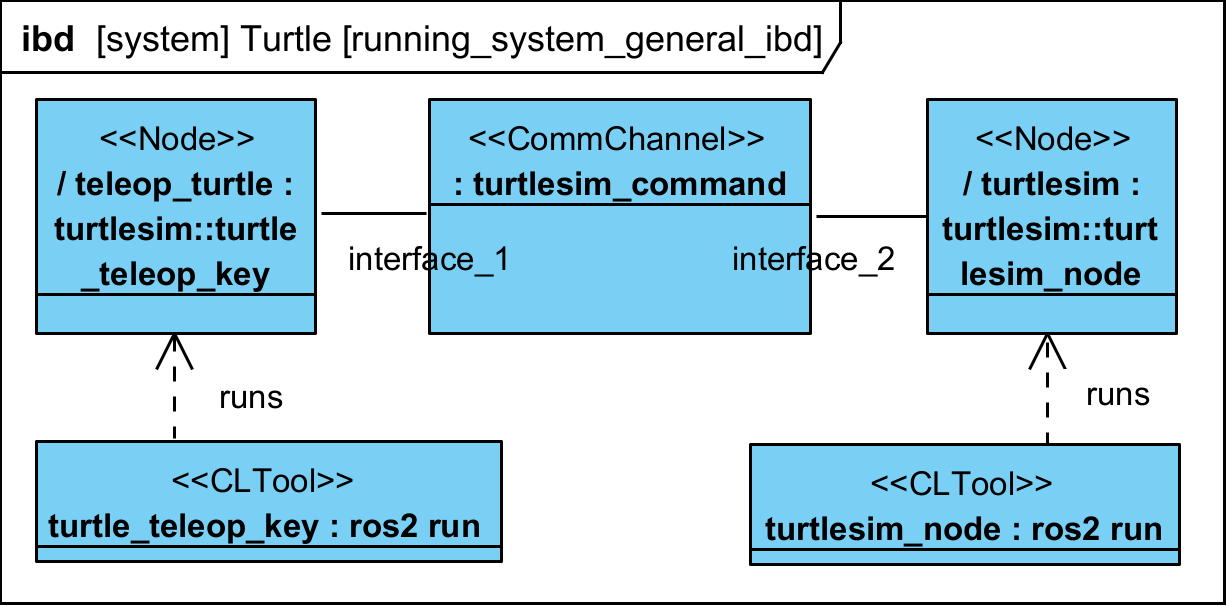
\includegraphics[scale=1.0]{diagrams/running_system_general_ibd.png}}
	\end{center}
	\caption{Running System general view ibd}
	\label{fig:running_system_general_ibd}
\end{figure}

\textsf{turtlesim\_command command} \stCommChannel{} is depicted in Fig.~\ref{fig:turtlesim_command_channel_bdd} and Fig.~\ref{fig:turtlesim_command_channel_ibd}. It should be noted that connector direction denote the publisher to subscriber data flow in case of \stTopic{}s or client to server in case of \stService{}s or \stAction{}s.


\begin{figure}[H]
	\centering
	\begin{center}
		{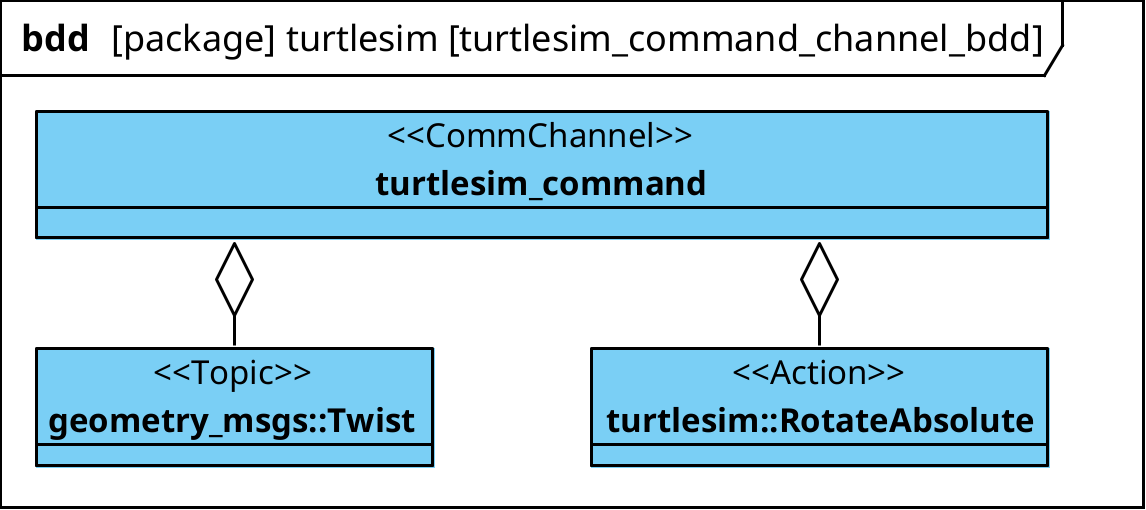
\includegraphics[scale=1.0]{diagrams/turtlesim_command_channel_bdd.png}}
	\end{center}
	\caption{turtlesim\_command command channel bdd}
	\label{fig:turtlesim_command_channel_bdd}
\end{figure}

\begin{figure}[H]
	\centering
	\begin{center}
		{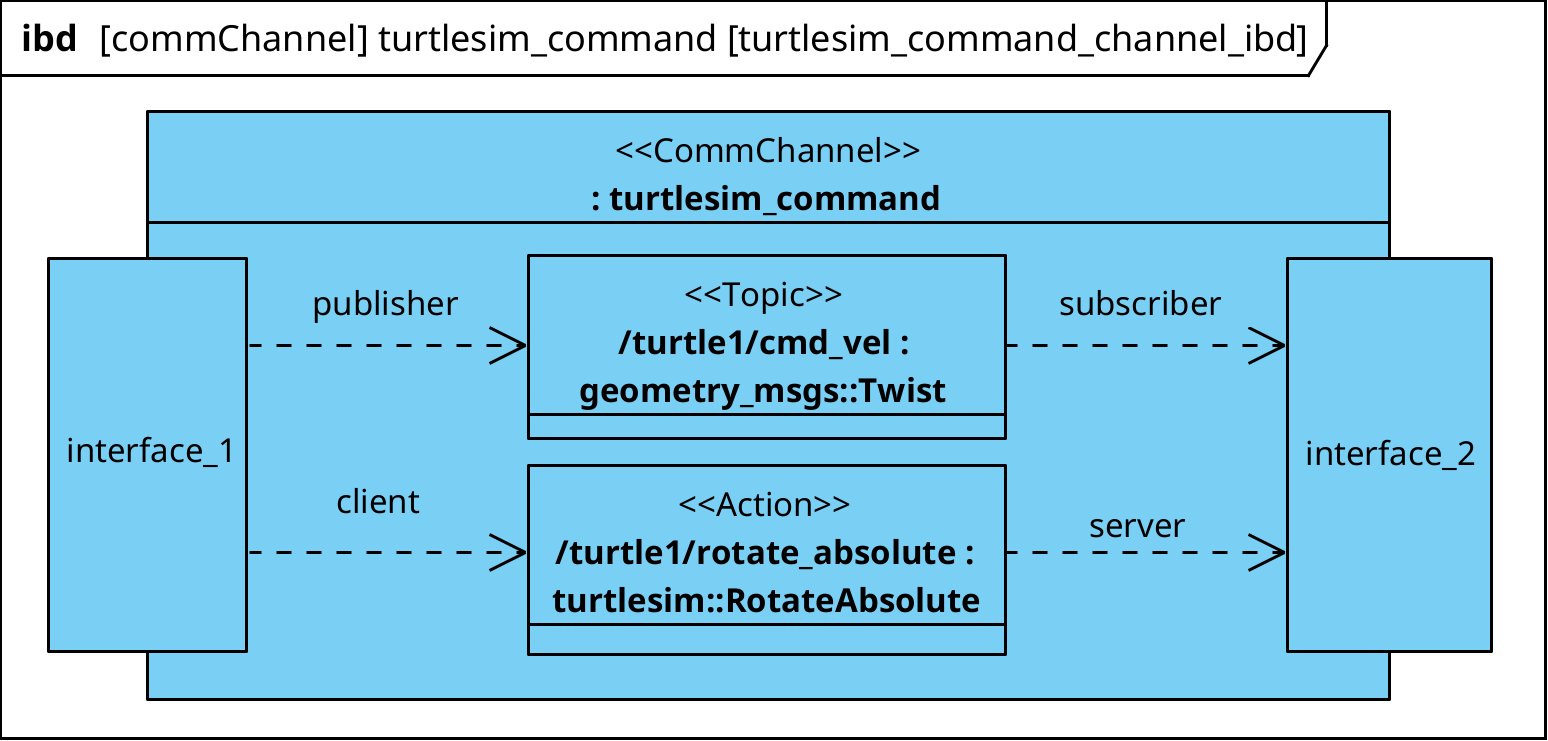
\includegraphics[scale=1.0]{diagrams/turtlesim_command_channel_ibd.png}}
	\end{center}
	\caption{turtlesim\_command command channel ibd}
	\label{fig:turtlesim_command_channel_ibd}
\end{figure}
			
\pagebreak			
			
The running system architecture can be also depicted in detailed way at once in Fig.~\ref{fig:running_system_detailed_bdd} and Fig.~\ref{fig:running_system_detailed_ibd}.
			
\begin{figure}[H]
	\centering
	\begin{center}
		{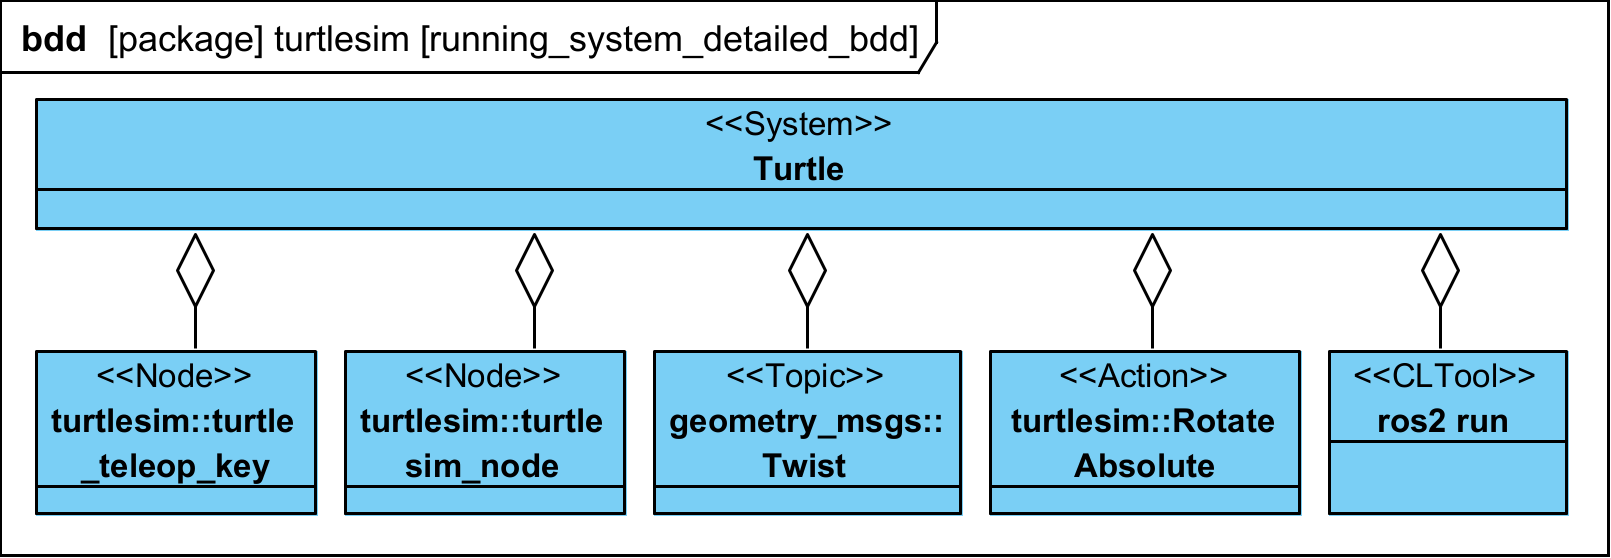
\includegraphics[scale=.9]{diagrams/running_system_detailed_bdd.png}}
	\end{center}
	\caption{Running System detailed view bdd}
	\label{fig:running_system_detailed_bdd}
\end{figure}

\begin{figure}[H]
	\centering
	\begin{center}
		{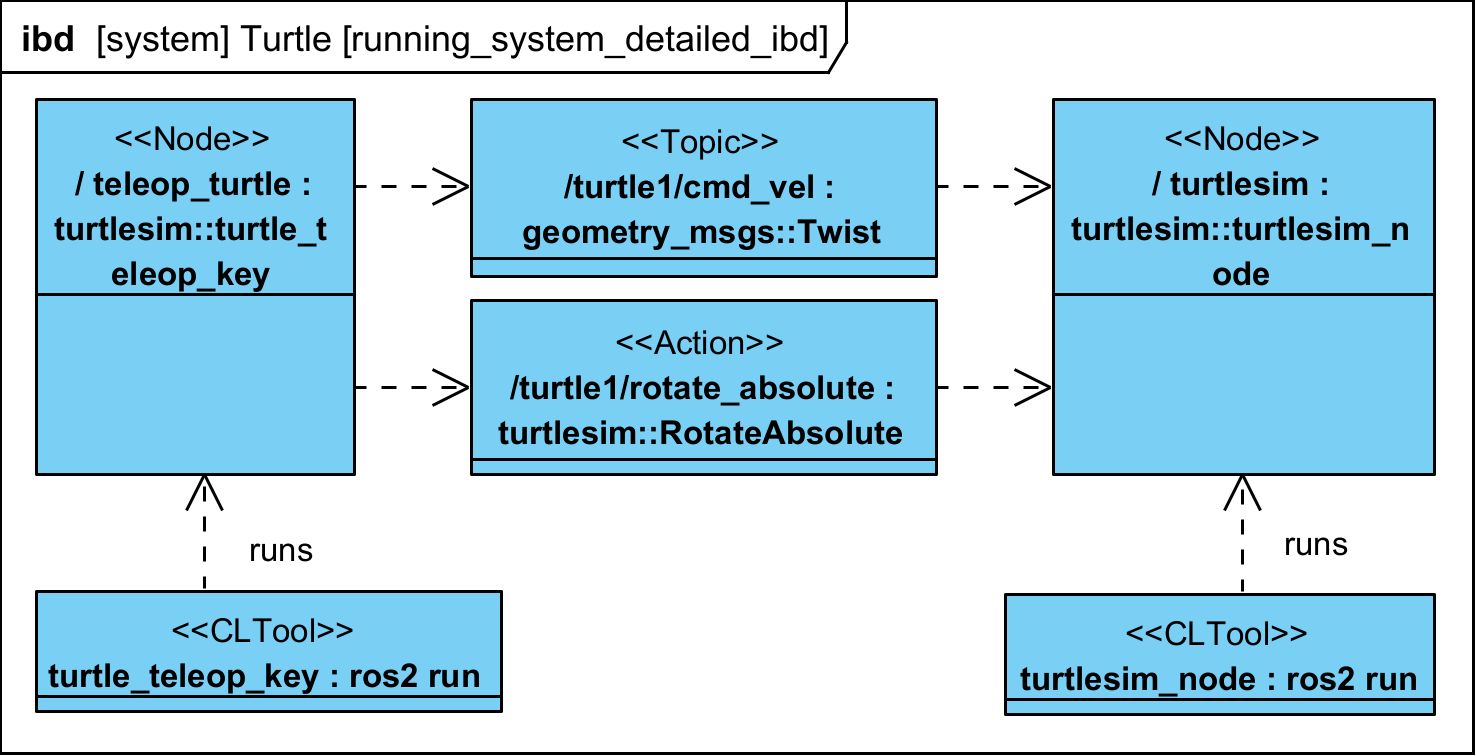
\includegraphics[scale=.9]{diagrams/running_system_detailed_ibd.png}}
	\end{center}
	\caption{Running System detailed view ibd}
	\label{fig:running_system_detailed_ibd}
\end{figure}
			
Now the detailed validation scenario can be presented (Fig.~ \ref{fig:detailed_scenario_sd}). It should be noted that \stAction{} call is depicted in one of the sequences that can occur during \stSystem{} execution.
			
\begin{figure}[H]
	\centering
	\begin{center}
		{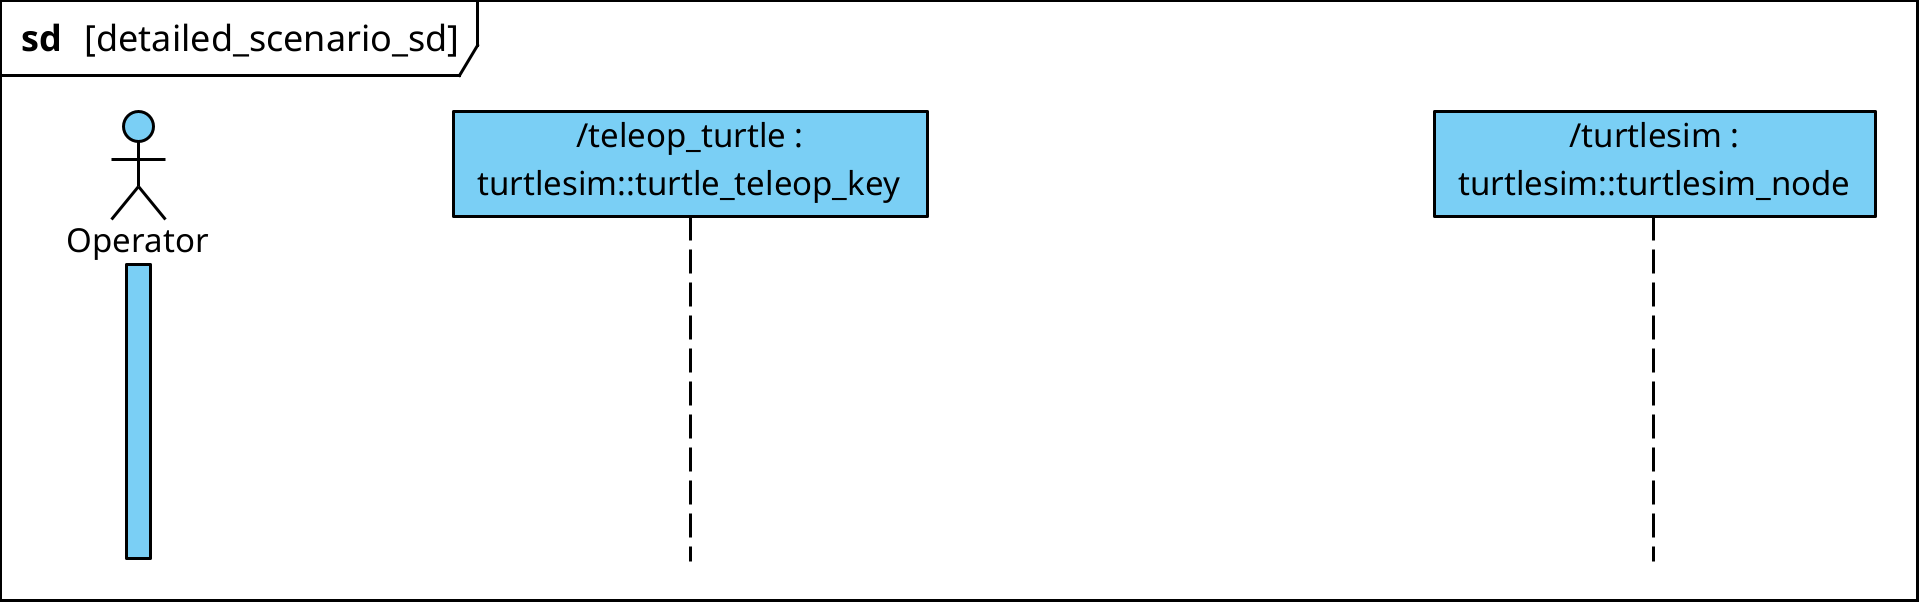
\includegraphics[scale=.9]{diagrams/detailed_scenario_sd.png}}
	\end{center}
	\caption{Running System detailed view ibd}
	\label{fig:detailed_scenario_sd}
\end{figure}
			
\AtNextBibliography{\small}
\printbibliography
	
\end{document}
